% !TeX program = lualatex
\documentclass[UTF8,a4paper,11pt,fontset=fandol]{ctexart}

\usepackage[a4paper,top=22mm,bottom=22mm,left=24mm,right=24mm]{geometry}
\usepackage{graphicx}
\usepackage[export]{adjustbox}
\usepackage[table]{xcolor}
\usepackage{booktabs,tabularx,array}
\usepackage[font=small,labelfont=bf,justification=centering,hypcap=false]{caption}
\usepackage{fvextra}
\usepackage[hidelinks]{hyperref}
\definecolor{ReportBlue}{HTML}{263F59}
\definecolor{ReportTint}{HTML}{EDF1F5}
\definecolor{ReportRule}{HTML}{6C8195}
\urlstyle{tt}
\setlength{\parindent}{2em}
\setlength{\parskip}{0pt}
\setlength{\tabcolsep}{5pt}
\renewcommand{\arraystretch}{1.16}
\pagestyle{plain}
\raggedbottom
\setlength{\emergencystretch}{1.5em}
\ctexset{
  section={format=\Large\bfseries\color{ReportBlue},beforeskip=1.1ex,afterskip=.8ex},
  subsection={format=\normalsize\bfseries\color{ReportBlue},beforeskip=1ex,afterskip=.5ex}
}
\DeclareCaptionFont{reportblue}{\color{ReportBlue}}
\captionsetup{labelfont={bf,reportblue}}
\DefineVerbatimEnvironment{Code}{Verbatim}{fontsize=\footnotesize,breaklines=true,frame=lines,framesep=2mm,rulecolor=\color{ReportRule}}
\newcolumntype{L}[1]{>{\raggedright\arraybackslash}p{#1}}
\newcolumntype{Y}{>{\raggedright\arraybackslash}X}
\newcommand{\thd}[1]{\multicolumn{1}{c}{\textcolor{ReportBlue}{\textbf{#1}}}}
\newcommand{\keypoint}[1]{\textcolor{ReportBlue}{\textbf{#1}}}
\newcommand{\code}[1]{\texttt{#1}}
\newcommand{\reportfigure}[3]{%
  \begin{center}
    \includegraphics[width=#1]{figures/#2}
    \captionof{figure}{#3}
  \end{center}}

\title{\heiti\color{ReportBlue}\fontsize{26}{34}\selectfont 深圳地铁数据库的设计与实现}
\author{舒石礼惠\quad 12511020 \qquad 黄斌鑫\quad 12411325}
\date{CS307 数据库原理课程项目一\quad 2026 年秋季学期}
\hypersetup{pdftitle={深圳地铁数据库的设计与实现},pdfauthor={舒石礼惠、黄斌鑫}}

\begin{document}
\maketitle

\begin{abstract}
本文基于深圳地铁车站与出口地标两份课程 CSV，设计并实现 PostgreSQL 数据库。概念模型区分物理车站、线路、行政区和出口，将站序、开通年份及首末班时间归入站线联系。关系模式由六张表组成，导入后包含 \keypoint{439 个物理车站、29 条线路}、1,304 个出口和 3,271 条出口地标关联。导入采用单事务和批量插入，并在装载后集中建立辅助索引。Java 应用通过 JDBC 提供车站及线路维护、站序调整、路径查询和地标查询。

\smallskip
\noindent\textbf{关键词：} 地铁数据库；实体联系模型；关系规范化；批量导入；路径查询
\end{abstract}

\section{项目概述与分工}

课程数据包含运营与在建线路。主 CSV 的一行表示某个车站在线路上的一次出现，同一物理车站可能属于多条线路。出口 CSV 则记录车站出口及附近地标，部分出口字段包含组合编号，地标字段也可包含多个名称。设计将这些不同粒度的记录分别组织，并通过主键、外键和唯一约束表达其对应关系。

\begin{center}
\captionof{table}{组员信息与贡献}
\small
\begin{tabularx}{\linewidth}{@{}llYc@{}}
\toprule
\rowcolor{ReportTint}
\thd{姓名} & \thd{学号} & \thd{工作分工} & \thd{贡献比例}\\
\midrule
舒石礼惠 & 12511020 & Task 1 概念模型、Task 2 关系模式、Task 3.1 数据准备与转换、Task 3.2 一键导入及性能优化。整理报告并核对图、DDL 和字段说明。 & 50\%\\
黄斌鑫 & 12411325 & Task 3.3 数据准确性核验与邻站函数、Task 4 增删改查、站序维护、路径与地标查询及本地界面。 & 50\%\\
\bottomrule
\end{tabularx}
\end{center}

两位组员均参加周一晚第 9--10 节实验课。数据库结构、数据装载与应用程序分别保存在 \path{sql/schema.sql}、\path{sql/import.sql} 和 \path{app/}。另有 10 个行政区及 567 条站线关系，六张表合计 5,620 行。

\clearpage
\section{概念模型（Task 1）}

\reportfigure{\linewidth}{concept-er.png}{深圳地铁概念 E-R 图（diagrams.net 绘制）}

行政区、车站和线路是强实体，主键用实线下划线表示。行政区与车站为一对多联系，每站恰属一个区。线路与车站为多对多联系，两端均允许暂时没有对应记录。\keypoint{站序、状态、开通年及首末班时间取决于站线组合}。例如，世界之窗在 Line 1、Line 2 的开通年分别为 2004、2010。

出口编号可在不同车站重复。\keypoint{出口由所属车站和部分键} \code{exit\_code} \keypoint{共同识别}。双矩形表示弱实体，双菱形表示识别联系，虚线下划线标记部分键，出口侧双线表示全参与。地标名称是出口的多值属性，允许为空。

\section{关系模式（Task 2）}

\reportfigure{\linewidth}{datagrip-schema.png}{PostgreSQL 六表关系图（DataGrip 导出）}

行政区与车站、车站与出口的联系通过外键实现。站线多对多联系形成 \code{line\_station}，出口的多值地标形成 \code{exit\_landmark}。出口保留 \code{(station\_id, exit\_code)} 作为业务候选键，并以整数 \code{exit\_id} 为主键，供地标关联表引用。完整建表语句随 \path{sql/schema.sql} 单独提供。

\clearpage
\subsection{字段及约束}

\begin{center}
\captionof{table}{六表字段字典}
\small
\begin{tabularx}{\linewidth}{@{}L{28mm}L{28mm}Y@{}}
\toprule
\rowcolor{ReportTint}
\thd{关系表} & \thd{字段} & \thd{类型、约束及含义}\\
\midrule
\textcolor{ReportBlue}{\code{district}} & \code{district\_id} & \code{integer}，自增主键，行政区编号。\\
 & \code{name\_en} & \code{text}，唯一，源数据的英文区名。\\
\addlinespace
\textcolor{ReportBlue}{\code{station}} & \code{station\_id} & \code{integer}，自增主键，物理车站编号。\\
 & \code{district\_id} & \code{integer}，外键，表示车站所属行政区。\\
 & \code{name\_zh} & \code{text}，中文站名，与区编号联合唯一。\\
 & \code{name\_en} & \code{text}，英文站名，允许同名。\\
 & \code{lon\_mdeg} & \code{integer}，可空，经度乘以 1,000，范围为 $\pm180{,}000$。\\
 & \code{lat\_mdeg} & \code{integer}，可空，纬度乘以 1,000，范围为 $\pm90{,}000$。经纬度同时为空或同时有值。\\
\addlinespace
\textcolor{ReportBlue}{\code{metro\_line}} & \code{line\_id} & \code{integer}，自增主键，区分支线和独立分期。\\
 & \code{name\_zh} & \code{text}，唯一，完整中文线路名称。\\
 & \code{name\_en} & \code{text}，唯一，完整英文线路名称。\\
\addlinespace
\textcolor{ReportBlue}{\code{line\_station}} & \code{line\_id} & \code{integer}，线路外键，与车站编号组成主键。\\
 & \code{station\_id} & \code{integer}，车站外键，与线路编号组成主键。\\
 & \code{position} & \code{integer}，正整数，表示源 \code{Num}。与线路编号联合唯一，约束可延迟检查。\\
 & \code{status} & \code{text}，车站在线路上的状态，取值为 \code{Operation} 或 \code{Construction}。\\
 & \code{opening\_year} & \code{smallint}，该站在该线的开通或预计开通年，范围为 1900--2200。\\
 & \code{first\_train} & \code{time(0)}，可空，该线该站的首班时间。\\
 & \code{last\_train} & \code{time(0)}，可空，该线该站的末班时间。\\
\addlinespace
\textcolor{ReportBlue}{\code{station\_exit}} & \code{exit\_id} & \code{integer}，自增主键，出口编号。\\
 & \code{station\_id} & \code{integer}，车站外键，删除车站时级联。\\
 & \code{exit\_code} & \code{text}，拆分后的出口代码，与车站编号联合唯一。\\
\addlinespace
\textcolor{ReportBlue}{\code{exit\_landmark}} & \code{exit\_id} & \code{integer}，出口外键，删除出口时级联。\\
 & \code{landmark\_name} & \code{text}，单个地标名，与出口编号组成主键。\\
\bottomrule
\end{tabularx}
\end{center}

除表中标注可空的字段外，其余字段均为非空。名称、出口码和地标名经过去空白检查。五条外键覆盖全部六表，引用方向无环。

\subsection{规范化分析}

\textbf{第一范式}通过拆分组合出口和地标集合保证字段原子性。\textbf{第二范式}要求站线表的站序、年份、状态及时间依赖完整的站线组合，地标关联表则没有非键字段。\textbf{第三范式}通过独立保存行政区、车站及线路名称消除传递依赖，站线关系只保存标识与关系属性。站序连续性由导入检查及插站、移站事务共同维护。

\clearpage
\section{数据导入（Task 3）}

\subsection{数据转换与辅助工具（Task 3.1）}

同名站使用中文名和行政区区分，保留龙岗和罗湖的两个梨园站。出口表的梨园 B/C 出口映射到龙岗站。组合出口拆分为独立代码，原行地标分配至组内各出口。经纬度按取值范围映射，源 \code{latitude} 对应经度，源 \code{longitude} 对应纬度。缺失的坐标和时刻以 \code{NULL} 保存。

\begin{center}
\captionof{table}{数据导入与核验工具}
\small
\begin{tabularx}{\linewidth}{@{}L{46mm}L{16mm}L{20mm}Y@{}}
\toprule
\rowcolor{ReportTint}
\thd{名称} & \thd{类型} & \thd{作者或使用者} & \thd{用途与调用方式}\\
\midrule
\path{tools/generate_import.py} & Python & 舒石礼惠 & 校验源文件并生成导入脚本。运行 \code{python tools/generate\_import.py}。\\
\path{sql/schema.sql}、\path{sql/indexes.sql} & SQL & 舒石礼惠 & 表结构与辅助索引，已合入完整导入脚本。\\
\path{sql/import.sql} & SQL & 舒石礼惠 & 一键导入，在 DataGrip 中执行整个文件。\\
\path{scripts/local-db.ps1} & PowerShell & 舒石礼惠 & 启动项目数据库并导入。调用 \code{-Action import} 装载数据。\\
\path{sql/functions.sql} & SQL & 黄斌鑫 & 定义 Q7 邻站函数，随导入建立。\\
\path{tools/verify_import.py} & Python & 黄斌鑫 & 校验导入内容、序列和约束。在验证库运行 \code{python tools/verify\_import.py --database} 后接库名。\\
\path{sql/queries.sql} & SQL & 黄斌鑫 & 在 DataGrip 或 psql 执行 Q1--Q7。\\
ChatGPT & LLM & 黄斌鑫 & 辅助 CSV 拆分、格式与查询口径检查。\\
Codex & AI 助手 & 舒石礼惠\newline 黄斌鑫 & 辅助核对数据、脚本及报告排版。\\
\bottomrule
\end{tabularx}
\end{center}

\subsection{一键导入与性能（Task 3.2）}

\path{sql/import.sql} 在一个事务内按外键依赖逆序清理旧表，再重建六表并按父表在前的顺序装载。每张表使用一条多值 \code{INSERT}，重建、装载、行数校验与统计更新由一个 \code{DO} 块执行。四个自增序列随后与最大编号对齐。辅助索引在写入数据后建立，事务失败时本轮重建回滚。

\begin{center}
\captionof{table}{导入脚本性能对比}
\small
\begin{tabular}{@{}lrr@{}}
\toprule
\rowcolor{ReportTint}
\thd{指标} & \thd{原脚本} & \thd{优化后}\\
\midrule
客户端执行的顶层语句数 & 48 & \keypoint{5}\\
多值 \code{INSERT} 条数 & 15 & 6\\
同连接 JDBC 导入中位数 & 765.8 ms & \keypoint{750.1 ms}\\
\bottomrule
\end{tabular}
\end{center}

在 PostgreSQL 12.1 上经同一 JDBC 连接交错运行两个版本各 15 次，优化后中位数下降约 2\%。DataGrip 两次完整执行优化版分别耗时 825 ms 与 586 ms。

\clearpage
\subsection{数据准确性查询（Task 3.3）}

在本机独立数据库执行 \path{sql/import.sql} 后，使用 psql 运行 \path{sql/queries.sql} 并记录结果。Q1、Q2 分别返回 \keypoint{439 站、29 线}。Q3 通过 \code{EXISTS} 避免重复统计换乘站。Q4 按 Line 5 的开通年份分组。Q5 使用左连接统计出口，保留并列第一的车站。

\begin{Code}[fontsize=\scriptsize]
-- Q1
SELECT count(*) AS station_count FROM project1.station;
-- Q2
SELECT count(*) AS line_count FROM project1.metro_line;
-- Q3
SELECT d.name_en AS district, count(*) AS cnt
FROM project1.station s JOIN project1.district d USING (district_id)
WHERE EXISTS (SELECT 1 FROM project1.line_station ls
              WHERE ls.station_id = s.station_id AND ls.status = 'Operation')
GROUP BY d.district_id, d.name_en ORDER BY d.name_en COLLATE "C";
-- Q4
SELECT ls.opening_year AS opening, count(*) AS cnt
FROM project1.line_station ls JOIN project1.metro_line l USING (line_id)
WHERE l.name_en = 'Line 5'
GROUP BY ls.opening_year ORDER BY ls.opening_year;
-- Q5
WITH counts AS (
    SELECT s.station_id, s.name_en AS english_name, count(e.exit_id) AS cnt
    FROM project1.metro_line l JOIN project1.line_station ls USING (line_id)
    JOIN project1.station s USING (station_id)
    LEFT JOIN project1.station_exit e USING (station_id)
    WHERE l.name_en = 'Line 1' GROUP BY s.station_id, s.name_en
)
SELECT english_name, cnt FROM counts WHERE cnt = (SELECT max(cnt) FROM counts)
ORDER BY english_name COLLATE "C";
\end{Code}

\begin{center}
\begin{tabular}{@{}c@{\hspace{4pt}}c@{\hspace{4pt}}c@{}}
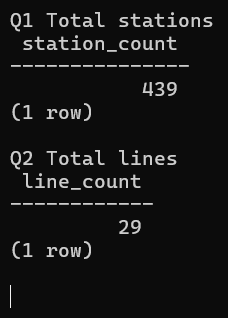
\includegraphics[scale=.38,valign=t]{figures/q1-q2.png} &
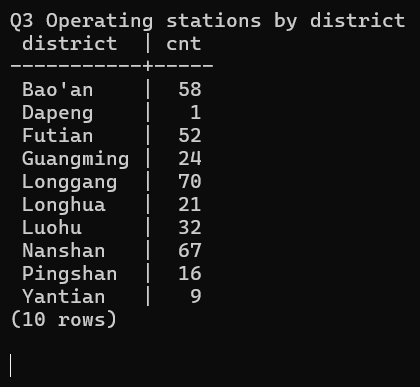
\includegraphics[scale=.38,valign=t]{figures/q3.png} &
\begin{tabular}[t]{@{}c@{}}
  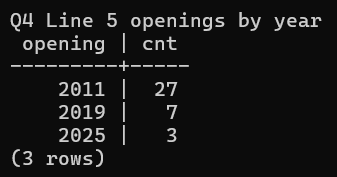
\includegraphics[scale=.38,valign=t]{figures/q4.png}\\[3pt]
  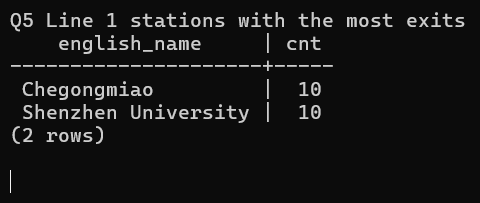
\includegraphics[scale=.38,valign=t]{figures/q5.png}
\end{tabular}
\end{tabular}
\captionof{figure}{Q1--Q5 本机 PostgreSQL 查询结果}
\end{center}

\clearpage
\subsection{地标前缀与邻站查询}

Q6 按地标名进行前缀匹配，按英文站名排序。Q7 按线路、站点和步长定位邻站，越界一侧以 \code{NULL} 表示。

\begin{Code}
-- Q6
SELECT s.name_zh AS chinese_name, d.name_en AS district,
       e.exit_code AS exit, el.landmark_name AS name
FROM project1.exit_landmark el JOIN project1.station_exit e USING (exit_id)
JOIN project1.station s USING (station_id)
JOIN project1.district d USING (district_id)
WHERE el.landmark_name LIKE '塘朗%'
ORDER BY s.name_en COLLATE "C", s.station_id,
         e.exit_code COLLATE "C", el.landmark_name COLLATE "C";
-- Q7
SELECT neighbor
FROM project1.get_station_n_neighbor('Mawan', 'Line 5', 5)
     WITH ORDINALITY AS t(neighbor, ord) ORDER BY ord;
SELECT project1.get_station_n_neighbor('Mawan', 'Line 5', 2);
\end{Code}

\begin{center}
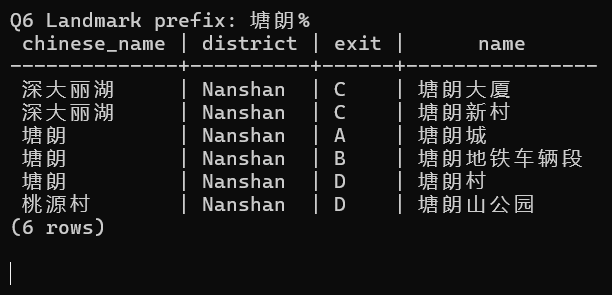
\includegraphics[scale=.45,valign=t]{figures/q6.png}\hspace{4pt}%
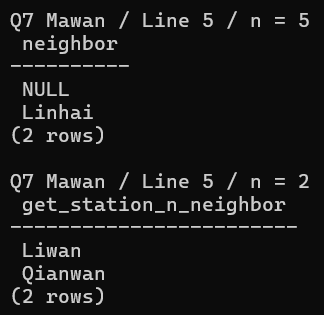
\includegraphics[scale=.45,valign=t]{figures/q7.png}
\captionof{figure}{Q6 地标前缀查询与 Q7 邻站查询的本机结果}
\end{center}

邻站函数由 \path{sql/functions.sql} 定义，按 \code{position}$-n$、\code{position}$+n$ 顺序返回两行。当 $n=0$ 时，两个位置均为本站。

\section{应用实现与部署（Task 4）}

\subsection{车站、线路及路径查询}

命令行与网页共用 Java 业务层，以 JDBC 参数绑定执行数据库操作。车站及线路支持新增、查询、修改和删除。批量插站先校验位置和站点，再后移其后的站序并按输入顺序插入。移站删除站线关系并重排站序。删除物理站时统一处理关联线路及出口。

路径查询以同线相邻站序构建双向图。\keypoint{最少站数}使用广度优先搜索。\keypoint{最少换乘}使用 Dijkstra 算法，换乘次数相同时按站数排序。地标查询先将两个地标映射为候选车站，再进行多起点、多终点搜索。票价接口从另行提供的 CSV 读取有向站对金额。

\clearpage
\subsection{Windows 部署流程}

\keypoint{安装依赖与建库。} 安装 \href{https://adoptium.net/installation}{JDK 17 或更新版本}并将其 \code{bin} 加入 PATH，再安装 \href{https://www.postgresql.org/download/windows/}{PostgreSQL 服务端与命令行工具}。将项目解压到可写目录，进入项目根目录。以下路径按本机安装位置填写。

\begin{Code}
Set-Location 'C:\work\Project1_v0'
$pgBin = 'C:\Program Files\PostgreSQL\18\bin'
java -version
javac -version
& "$pgBin\psql.exe" --version
.\scripts\local-db.ps1 -Action start -PgBin $pgBin
.\scripts\local-db.ps1 -Action import -PgBin $pgBin
.\scripts\build.ps1
java -jar app/build/metro.jar --action q1
java -jar app/build/metro.jar --action q2
.\scripts\run.ps1
# Web：在另一个 PowerShell 窗口进入同一项目目录后运行
.\scripts\run.ps1 -Web
\end{Code}

\keypoint{导入与核验。} \code{start} 初始化 \path{.runtime/pgdata}，创建数据库 \code{metro\_test}。\code{import} 建立 \code{project1}、载入数据并配置网页查询账号。\code{build.ps1} 生成 \path{app/build/metro.jar}。Q1、Q2 应分别返回 439 和 29。首次搭建或重置数据时执行导入。

\keypoint{启动与访问。} 浏览器地址为 \url{http://127.0.0.1:8088/}。在 DataGrip 中连接本机的 55437 端口，库名为 \code{metro\_test}，用户为 \code{metro}，密码留空。若数据库端口冲突，给 \code{start} 和 \code{import} 指定同一 \code{-Port}，并将 \code{METRO\_DB\_URL} 设置为对应 JDBC 地址。

\begin{center}
\begin{minipage}[t]{.51\linewidth}
  \centering
  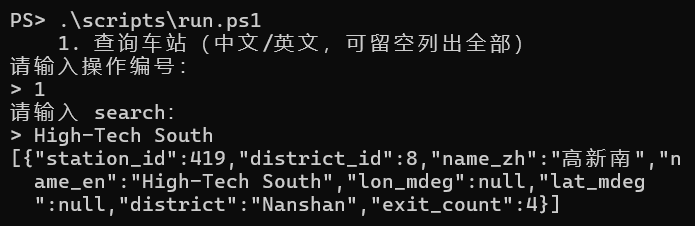
\includegraphics[width=\linewidth,valign=t]{figures/cli.png}
  \captionof{figure}{命令行车站查询（菜单节选）}
\end{minipage}\hfill
\begin{minipage}[t]{.47\linewidth}
  \centering
  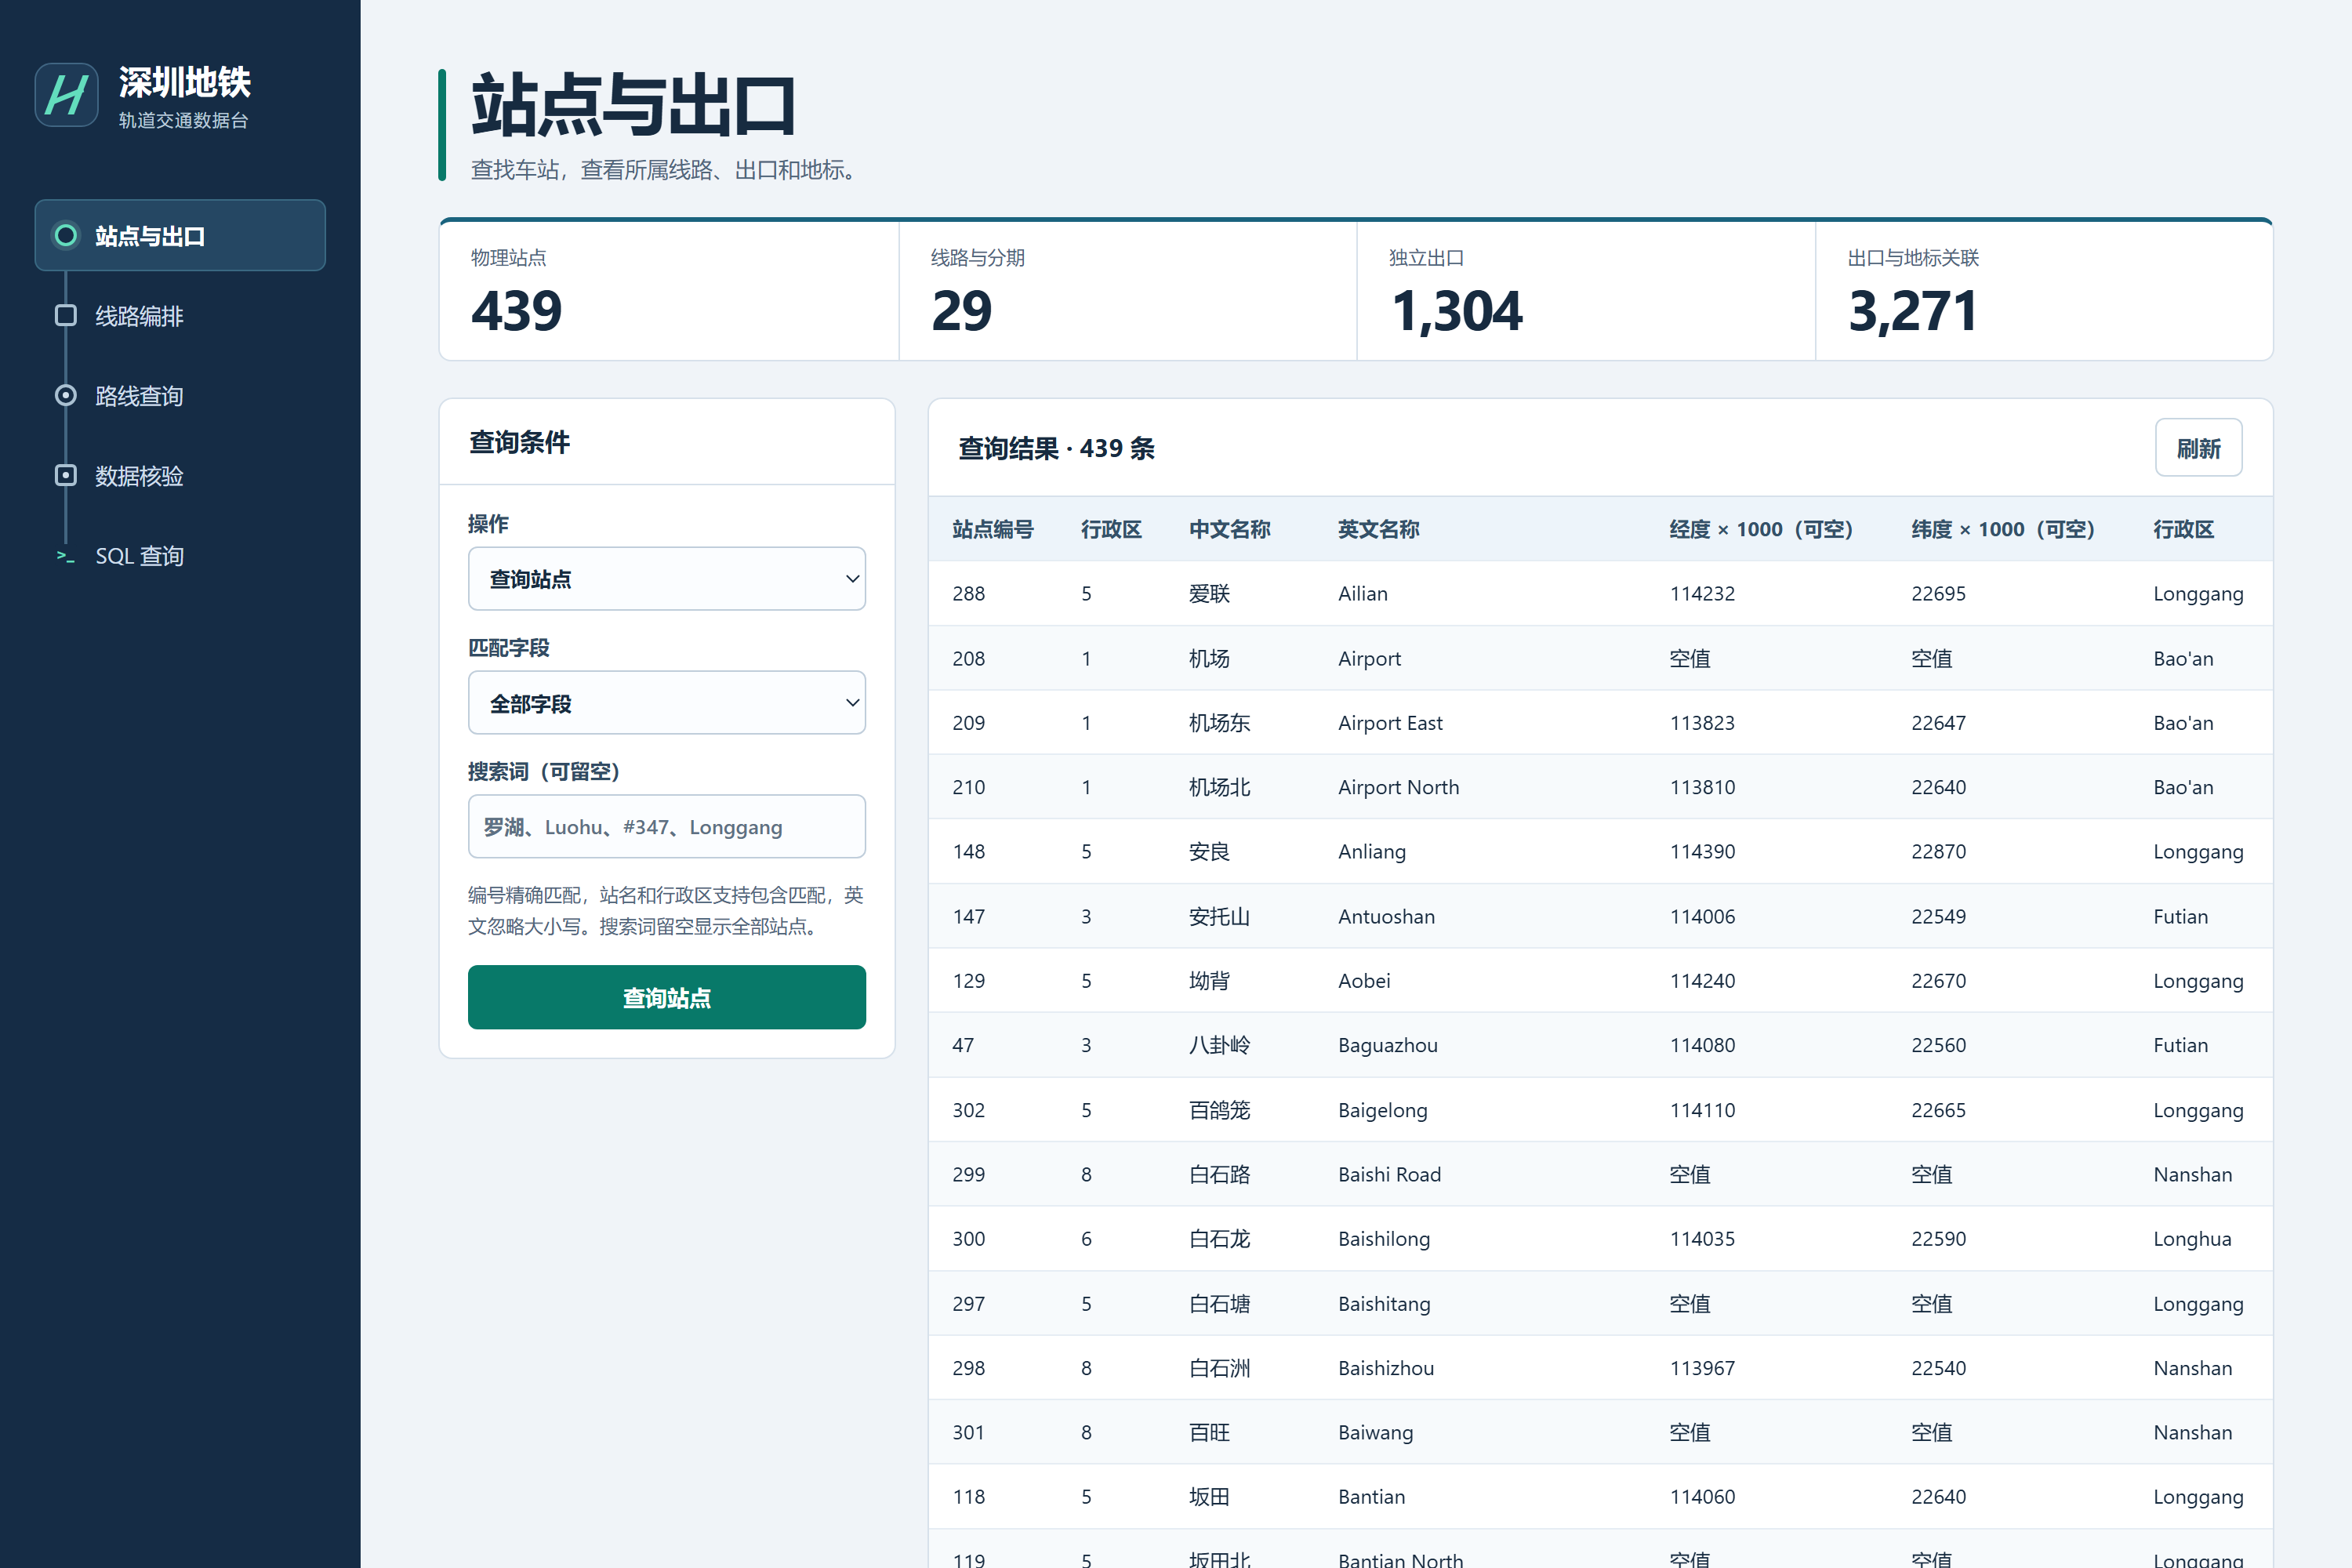
\includegraphics[width=\linewidth,valign=t]{figures/application.png}
  \captionof{figure}{网页车站查询界面}
\end{minipage}
\end{center}

\end{document}
